\documentclass{beamer}

\usepackage{pri}

\graphicspath{{./}{figures/}{figures/15-recommender-figs/}}

\subtitle{Recommender Systems}


\begin{document}

\maketitle

% ------------------------------------------------------------

\makeoutline

\begin{frame}
    \frametitle{Bibliography}
    \begin{block}{}
        \begin{itemize}
        \item \href{http://ijcai-11.iiia.csic.es/program/tutorials}{Dietmar
              Jannach and Gerhard Friedrich, \textit{Tutorial: Recommender
                Systems}, International Joint Conference on Artificial
              Intelligence Barcelona, 2011.}
        \item Francesco Ricci, Lior Rokach and Bracha Shapira,
            \textit{Recommender Systems Handbook}, Springer, 2011.
        \end{itemize}
    \end{block}
\end{frame}

\section{Introduction}

\begin{frame}
    \frametitle{What is a Recommender System?}
    \begin{block}{Recommender System}
        Recommender Systems (RS) are software tools and techniques providing
        suggestions for items to be of use to a user.
    \end{block}
    \vsep
    RS help to match users with items
    \begin{itemize}
    \item books, movies, music, travel, consumer products, news, ...
    \end{itemize}
\end{frame}

\begin{frame}
    \frametitle{Examples}
    \begin{columns}
        \column{.5\linewidth}
        \centering Amazon\\
        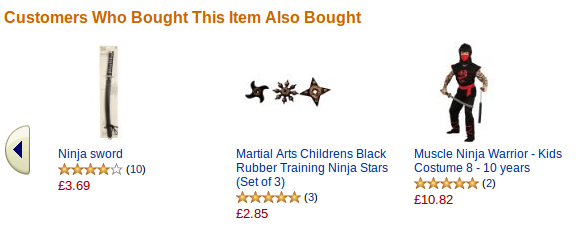
\includegraphics[width=\linewidth]{amazon}\\[\baselineskip]
        \centering Criticker\\
        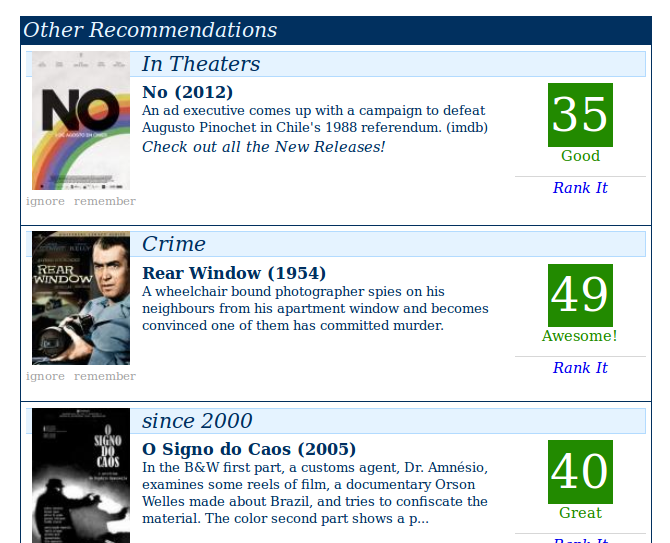
\includegraphics[width=\linewidth]{criticker}
        \column{.5\linewidth}
        \centering Goodreads\\
        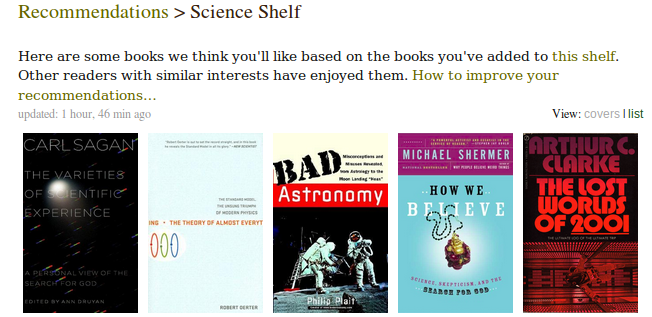
\includegraphics[width=\linewidth]{goodreads}\\[\baselineskip]
        \centering Grooveshark\\
        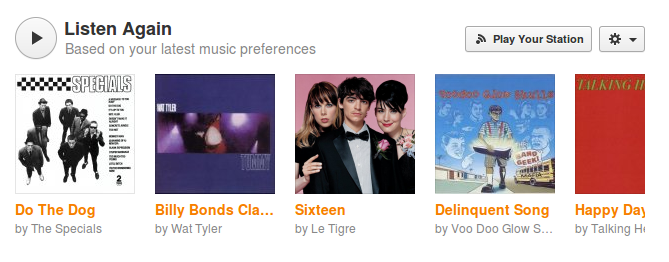
\includegraphics[width=\linewidth]{grooveshark}
    \end{columns}
\end{frame}

\begin{frame}
    \frametitle{Why Use Recommender Systems?}
    For users:
    \begin{itemize}
    \item Ease information overload
    \item Sales assistance
    \end{itemize}
    \vsep
    For providers:
    \begin{itemize}
    \item Can have high commercial value
        \begin{itemize}
        \item See, for example, the
            \emph{\href{http://www.netflixprize.com/}{\underline{Netflix
                  Prize}}}
        \end{itemize}
    \end{itemize}
\end{frame}

\begin{frame}
    \frametitle{Why Use Recommender Systems? (cont.)}
    Leverage the \emph{long tail}
    \begin{columns}
        \column{.5\linewidth}
        \begin{center}
            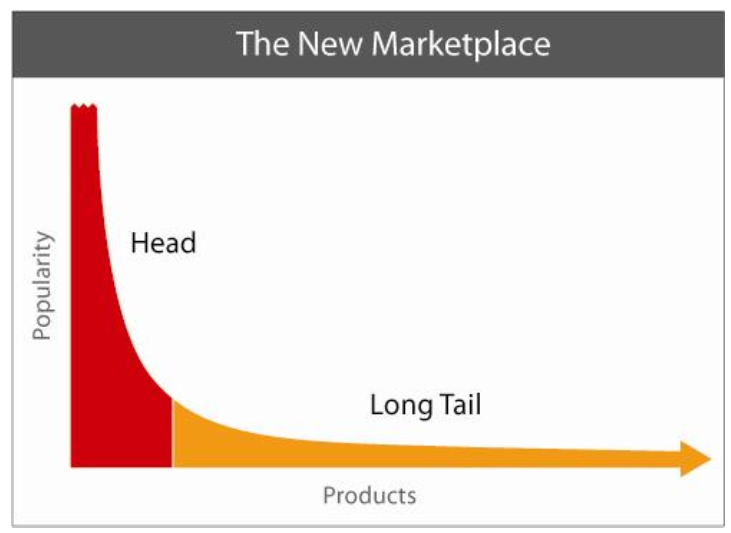
\includegraphics[width=\linewidth]{long-tail}
        \end{center}
        \column{.5\linewidth} \footnotesize (...) our culture and economy is
        increasingly shifting away from a focus on a relatively small number of
        "hits" (mainstream products and markets) at the head of the demand
        curve and toward a huge number of niches in the tail.
    \end{columns}
    \vsep
    \small Chris Anderson, \textit{The Long Tail: Why the Future of Business is
      Selling Less of More}, 2004.
\end{frame}

\begin{frame}[shrink]
    \frametitle{Goals of a Recommender System}
    \begin{itemize}
    \item \textbf{Retrieval:}
        \begin{itemize}
        \item Reduce search costs
        \item Provide accurate proposals
        \end{itemize}
    \item \textbf{Recommendation:}
        \begin{itemize}
        \item Serendipity --- identify items not known to the users
        \end{itemize}
    \item \textbf{Prediction:}
        \begin{itemize}
        \item Predict to what degree users like an item --- most popular
            evaluation scenario in research
        \end{itemize}
    \item \textbf{Interaction:}
        \begin{itemize}
        \item Give users a ``good feeling''
        \item Educate users about the product domain
        \item Convince/persuade users --- explain
        \end{itemize}
    \item \textbf{Commercial:}
        \begin{itemize}
        \item Increase \emph{hit}, \emph{clickthrough}, \emph{lookers to
              bookers} rates
        \item Optimize sales margins and profit
        \end{itemize}
    \end{itemize}
\end{frame} 

\begin{frame}
    \frametitle{How Recommendation Works}
    \begin{block}{Recommender System}
        \begin{description}
        \item[\textbf{Input:}]
            \emph{User model}: ratings, preferences, demographics, ...\\
            \emph{Items} (with or without description of item characteristics)
        \item[\textbf{Output:}] \emph{Relevance score}
        \end{description}
    \end{block}
    In practice, usually not all items will be scored: the task is to
    \emph{find the most relevant} ones.
\end{frame}

\newcommand{\insparadigm}[1]{\includegraphics<+>[trim=450 110 210 220, clip,
  width=\linewidth]{#1}}

\begin{frame}
    \frametitle{Paradigms of Recommender Systems}
    \centering
    \vsep
    \insparadigm{parad1}
    \insparadigm{parad2}
    \insparadigm{parad3}
    \insparadigm{parad4}
    \insparadigm{parad5}
    \insparadigm{parad6}
\end{frame}

\section{Collaborative Filtering}

\begin{frame}
    \frametitle{Collaborative Filtering (CF)}
    \begin{itemize}
    \item The most prominent approach to generate recommendations
        \begin{itemize}
        \item Used by large e-commerce sites
        \item Well-understood: various algorithms and variations exist
        \item Applicable in many domains (book, movies, DVDs, ..)
        \end{itemize}
    \item Approach
        \begin{itemize}
        \item Use the \emph{wisdom of the crowd} to recommend items
        \end{itemize}
    \item Basic assumption and idea
        \begin{itemize}
        \item Users give ratings to catalog items (implicitly or explicitly)
        \item Customers who had similar tastes in the past, will have similar
            tastes in the future
        \end{itemize}
    \end{itemize}
\end{frame}

\begin{frame}
    \frametitle{How CF works}
    \textbf{An example:} user-based nearest-neighbor collaborative filtering

    Given an \emph{active user} (Alice) and an item \emph{$I$} not yet seen by
    Alice
    \begin{itemize}
    \item<+-> The goal is to estimate Alice's rating for this item
        \begin{itemize}
        \item<+-> find a set of users (peers) who \emph{liked the same items} as
            Alice in the past \emph{and who have rated item $I$}
        \item<+-> use, e.g. the average of their ratings to predict if Alice
            will like item $I$
        \item<+-> do this for all items Alice has not seen and recommend the
            best-rated
        \end{itemize}
    \end{itemize}
    \hfill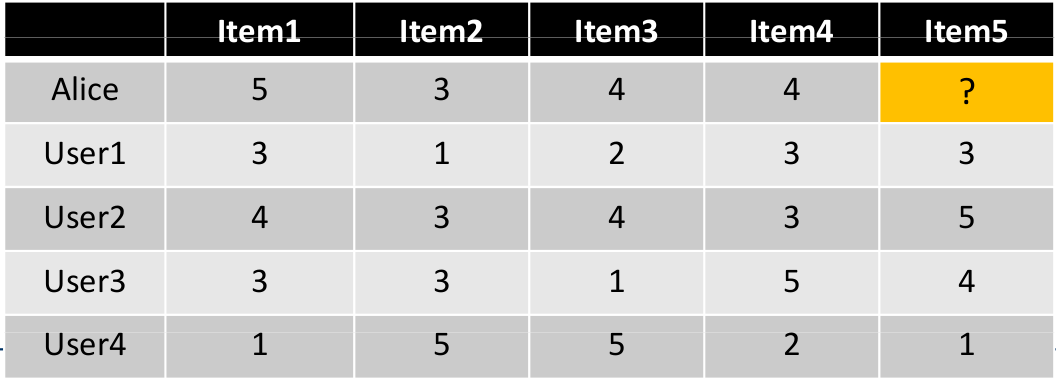
\includegraphics[width=.8\linewidth]{cf}\hfill~
\end{frame}

\begin{frame}
    \frametitle{How CF Works (cont.)}
    Some first questions:
    \begin{itemize}
    \item How do we measure similarity?
    %\item How many neighbors should we consider?
    \item How do we generate a prediction from the neighbors' ratings?
    \end{itemize}
    \hfill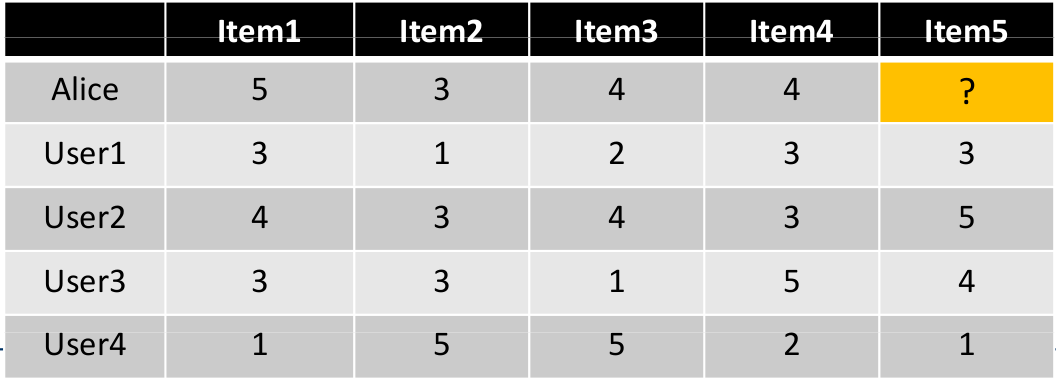
\includegraphics[width=.8\linewidth]{cf}\hfill~
\end{frame}

\begin{frame}
    \frametitle{Measuring User Similarity}
    \begin{block}{An example: Pearson correlation}
        \begin{displaymath}
            sim(a,b) = \frac{\sum_{p \in P}(r_{a,p}-\overline{r}_a)(r_{b,p}-\overline{r}_b)}{\sqrt{\sum_{p \in P}(r_{a,p}-\overline{r}_a)^2}\sqrt{\sum_{p \in P}(r_{b,p}-\overline{r}_b)^2}}
        \end{displaymath}
        \centering
        \begin{minipage}{0.7\linewidth}
            \footnotesize
            $a,b$: users\\
            $r_{a,p}$: rating of user $a$ for item $p$\\
            $P$: set of items, rated both by $a$ and $b$\\
            $\overline{r}_a,\overline{r}_b$ user's average ratings\\
            Possible similarity values between -1 and 1;
        \end{minipage}
    \end{block}
    \hfill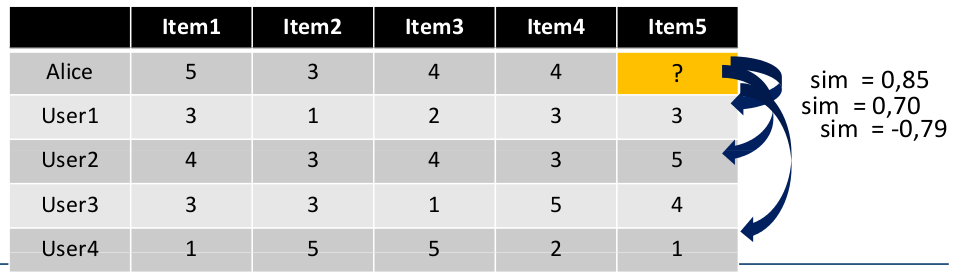
\includegraphics[width=\linewidth]{pearson}\hfill~
\end{frame}

\begin{frame}
    \frametitle{Pearson Correlation}
    \begin{itemize}
    \item Takes differences in rating behavior into account
    \end{itemize}
    \hfill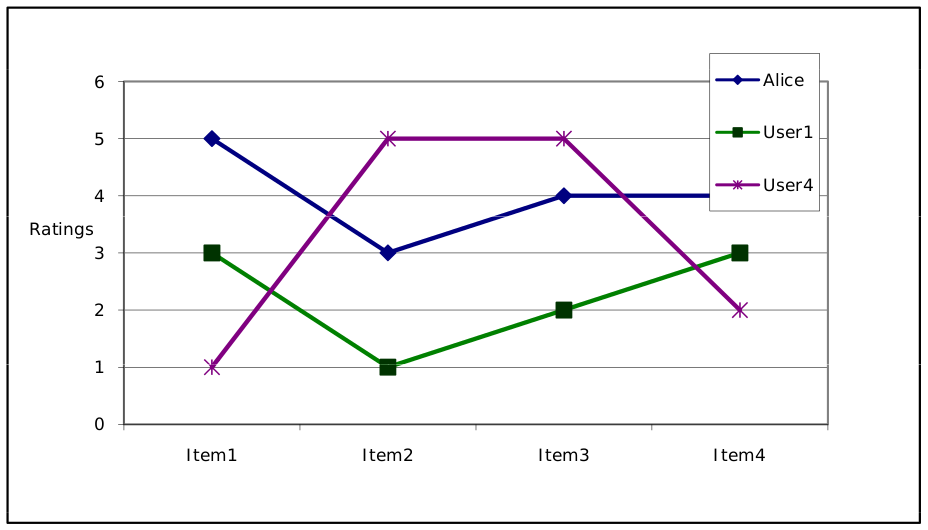
\includegraphics[width=.8\linewidth]{pearson2}\hfill~
    \begin{itemize}
    \item Works well in usual domains, compared with alternative measures
        \begin{itemize}
        \item such as cosine similarity
        \end{itemize}
    \end{itemize}
\end{frame}

\begin{frame}
    \frametitle{Making Predictions}
    \begin{itemize}
    \item A common prediction function:
        \begin{block}{}
            \begin{displaymath}
                pred(a,p) = \overline{r}_a + \frac{\sum_{b \in N}sim(a,b) \times (r_{b,p}-\overline{r}_b)}{\sum_{b \in N}sim(a,b)}
            \end{displaymath}
        \end{block}
    \item Calculate, whether the neighbors' ratings for the unseen item $p$ are
        higher or lower than their average
    \item Combine the rating differences: use the similarity with as a weight
    \item Add/subtract the neighbors' bias from the active user's average and
        use this as a prediction
    \end{itemize}
\end{frame}

% \begin{frame}
%     \frametitle{Improving the Metrics and Prediction}
%     \begin{itemize}
%         % Herlocker J, Konstan J, Borchers A and Riedl J (1999) An algorithmic
%         % framework for performing collaborative filtering. In: Proc. of
%         % Research and Development in Information Retrieval.
%     \item<+-> Not all neighbor ratings might be equally valuable
%         \begin{itemize}
%         \item<+-> Agreement on commonly liked items is not so informative as
%             agreement on controversial items
%         \item<+-> \emph{Solution:} Give more weight to items that have a higher
%             variance (\emph{variance weighting)}
%             \footnotesize
%             \begin{displaymath}
%                 sim(a,b) = \frac{\sum_{p \in P}v_p(r_{a,p}-\overline{r}_a)(r_{b,p}-\overline{r}_b)}{\sqrt{\sum_{p \in P}v_p(r_{a,p}-\overline{r}_a)^2}\sqrt{\sum_{p \in P}v_p(r_{b,p}-\overline{r}_b)^2}}
%             \end{displaymath}
%         \end{itemize}
%     \item<+-> Not all similarites should be equally trusted
%         \begin{itemize}
%         \item<+-> \emph{Solution:} impose a threshold of co-rated items
%         \item<+-> and/or reduce the weight when the number of co-rated items is
%             low (\emph{significance weighting})
%         \item<+-> E.g. $sim(a,b)' = \frac{n}{50}sim(a,b)$, where $n \leq 50$ is
%             the number of co-rated items
%         \end{itemize}
%     \end{itemize}
% \end{frame}

% \begin{frame}
%     \frametitle{Improving the Metrics and Prediction (cont.)}
%     \begin{itemize}
%     \item<+-> Similarity should not be linear
%         \begin{itemize}
%         \item<+-> \emph{Solution:} Give more weight to very similar neighbors
%             (\emph{case amplification})
%         \item<+-> E.g. $sim'(a,b) = sim(a,b)|sim(a,b)|^{\rho-1} $, $\rho \geq
%             1$
%             % Breese JS, Heckerman D and Kadie C (1998) Empirical analysis of
%             % predictive algorithms for collaborative filtering. Technical
%             % report, Microsoft Research.
%         \item<+-> Tends to favor close neighbors, as small values raised to a
%             power become negligible
%         \end{itemize}
%     \item<+-> Must limit the number of neighbours
%         \begin{itemize}
%         \item<+-> \emph{Solution:} Use similarity threshold
%         \item<+-> Or a fixed number of neighbors
%         \end{itemize}
%     \end{itemize}
% \end{frame}

\begin{frame}
    \frametitle{Memory-based and Model-based Approaches}
    \begin{itemize}
    \item User-based CF is said to be \emph{memory-based}
        \begin{itemize}
        \item the rating matrix is directly used to find neighbors and make
            predictions
        \item hard to scale for most real-world scenarios: large e-commerce
            sites have tens of millions of customers and millions of items
        \end{itemize}
    \item \textbf{Model-based approaches}
        \begin{itemize}
        \item based on an offline pre-processing or \emph{model-learning} phase
        \item at run-time, only the learned model is used to make predictions
        \item models are updated periodically (can be computationally
            expensive)
        \item large variety of techniques used
        \end{itemize}
    \end{itemize}
\end{frame}

\begin{frame}
    \frametitle{Issues with User-based CF}
    \begin{itemize}
    \item Scalability issues arise if there are many more users than items
        \begin{itemize}
        \item e.g. amazon.com
        \item Space complexity $O(m^2)$, when pre-computed
        \item Time complexity for computing Pearson: $O(m^2n)$
        \end{itemize}
    \item High sparsity leads to few common ratings between two users
    \item A solution: \emph{Item-based CF}
        \begin{itemize}
        \item exploits relationships between items, instead of relationships
            between users
        \end{itemize}
    \end{itemize}
\end{frame}

\begin{frame}
    \frametitle{Item-based Collaborative Filtering}
    \begin{itemize}
    \item \textbf{Basic idea:} Use the similarity between items (and not users)
        to make predictions
    \item Example:
        \begin{itemize}
        \item Look for items that are similar to Item5
        \item Take Alice's ratings for these items to predict the rating for
            Item5
        \end{itemize}
    \end{itemize}
    \hfill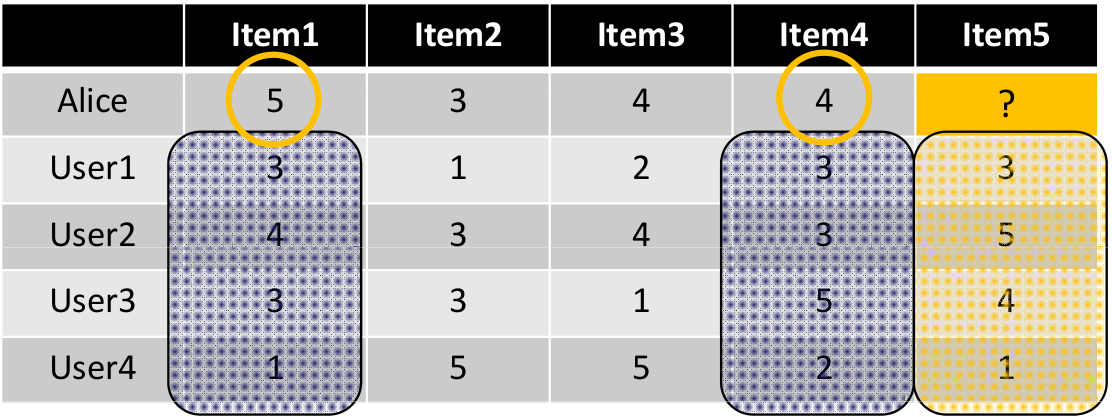
\includegraphics[width=.8\linewidth]{itemCF}\hfill~
\end{frame}

\begin{frame}
    \frametitle{The Cosine Similarity Measure}
    \begin{itemize}
    \item  Produces better results in item-to-item filtering
        \begin{itemize}
        \item (for some datasets)
        \end{itemize}
    \item Ratings are seen as vector in n-dimensional space
    \item Similarity is calculated based on the angle between the vectors
        \begin{displaymath}
                sim(a,b) = \frac{\sum_{u \in U}r_{u,a}r_{u,b}}{\sqrt{\sum_{u \in U}r_{u,a}^2}\sqrt{\sum_{u \in U}r_{u,b}^2}}
        \end{displaymath}
    \item Adjusted cosine similarity
        \begin{itemize}
        \item take average user ratings into account, transform the original
            ratings
            \begin{displaymath}
                sim(a,b) = \frac{\sum_{u \in U}(r_{u,a}-\overline{r}_u)(r_{u,b}-\overline{r}_u)}{\sqrt{\sum_{u \in U}(r_{u,a}-\overline{r}_u)^2}\sqrt{\sum_{u \in U}(r_{u,b}-\overline{r}_u)^2}}
            \end{displaymath}
        \item $U$: set of users who have rated both items $a$ and $b$
        \end{itemize}
    \end{itemize}
\end{frame}

\begin{frame}
    \frametitle{Pre-processing for Item-based CF}
    \begin{itemize}
    \item Item-based CF does not solve the scalability problem itself
    \item Pre-processing approach by Amazon.com (in 2003)
        \begin{itemize}
        \item Calculate all pair-wise item similarities in advance
        \item The neighborhood to be used at run-time is typically rather
            small, because only items are taken into account which the user has
            rated
        \item Item similarities are supposed to be more stable than user
            similarities
        \end{itemize}
    \item Memory requirements
        \begin{itemize}
        \item Up to $N^2$ pair-wise similarities to be memorized ($N$ = number
            of items) in theory
        \item In practice, this is significantly lower (items with no
            co-ratings)
        \item Further reductions possible
            \begin{itemize}
            \item Minimum threshold for co-ratings (items, which are rated at
                least by n users)
            \item Limit the size of the neighborhood (might affect
                recommendation accuracy)
            \end{itemize}
        \end{itemize}
    \end{itemize}
\end{frame}

\begin{frame}
    \frametitle{Data sparsity problems}
    \begin{itemize}
    \item<+-> \emph{Cold start problem}
        \begin{itemize}
        \item How to recommend new items? What to recommend to new users?
        \end{itemize}
    \item<+-> Straightforward approaches
        \begin{itemize}
        \item Ask/force users to rate a set of items
        \item Use another method (e.g., content-based, demographic or simply
            non-personalized) in the initial phase
        \end{itemize}
    \item<.-> Alternatives
        \begin{itemize}
        \item Use other algorithms (beyond nearest-neighbor approaches)
        \item Example:
            \begin{itemize}
            \item In nearest-neighbor approaches, the set of sufficiently
                similar neighbors might be to small to make good predictions
            \item Assume \emph{transitivity} of neighborhoods
            \end{itemize}
        \end{itemize}
    \end{itemize}
\end{frame}

\begin{frame}
    \frametitle{SVD: an approach to the sparsity problem}
    \begin{itemize}
    \item Basic idea: Trade more complex offline model building for faster
        online prediction generation
    \item \emph{Singular Value Decomposition} for dimensionality reduction of
        rating matrices
        \begin{itemize}
        \item Captures important factors and their weights in the data
        \item Assumption that $k$ dimensions capture the signals and filter out
            noise ($K =$ 20 to 100)
        \end{itemize}
    \item Constant time to make recommendations
    \item Approach also popular in IR (Latent Semantic Indexing)%, data compression,...
    \end{itemize}
\end{frame}

\begin{frame}
    \frametitle{How it works}
    For any matrix $A_{nm}$:
    \begin{displaymath}
        A_{mn} = U_{mm} \times S_{mn} \times V_{nn}^T
    \end{displaymath}
    \begin{itemize}
    \item $U^TU = I$, $V^TV = I$ (i.e. $U$ and $V$ are \emph{orthogonal} matrices)
    \item columns of $U$: orthonormal eigenvectors of $AA^T$
    \item columns of $V$: orthonormal eigenvectors of $A^TA$
    \item $S$: diagonal matrix containing the square roots of eigenvalues from
        U or V \emph{in descending order}
    \end{itemize}
    \vfill
    \scriptsize You can read about it here: \href{http://www.ling.ohio-state.edu/~kbaker/pubs/Singular_Value_Decomposition_Tutorial.pdf}{Kirk Baker, ``Singular Value
      Decomposition Tutorial'', 2005.}
\end{frame}

\begin{frame}
    \frametitle{How it works (cont.)}
    \begin{overprint}
        \centering
        \onslide<1>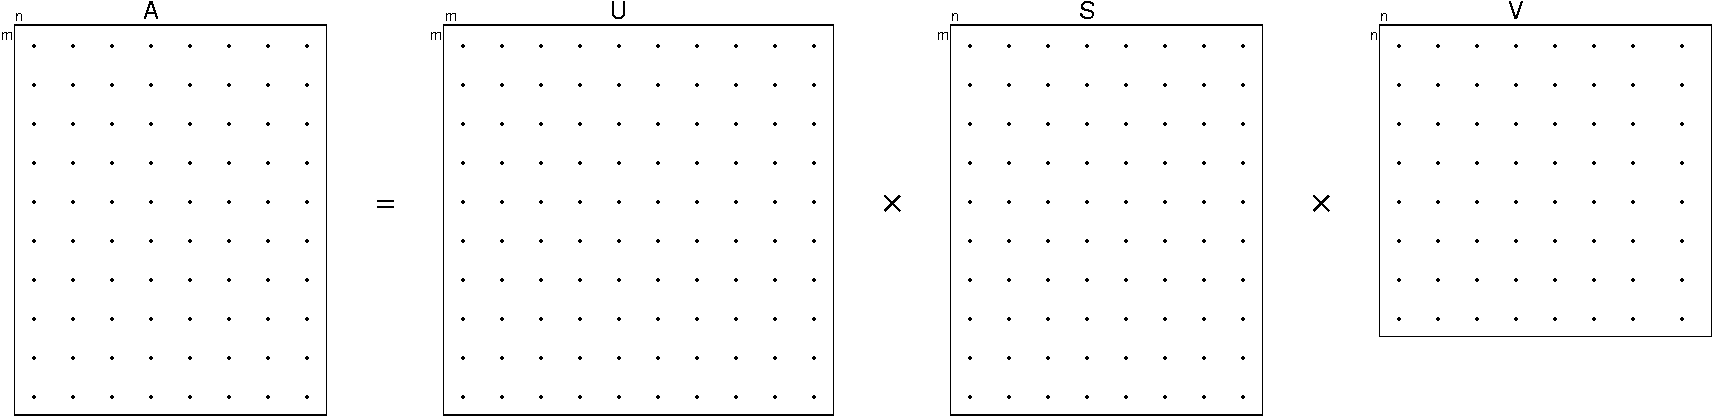
\includegraphics[width=\linewidth]{svdmatrix}
        \onslide<2>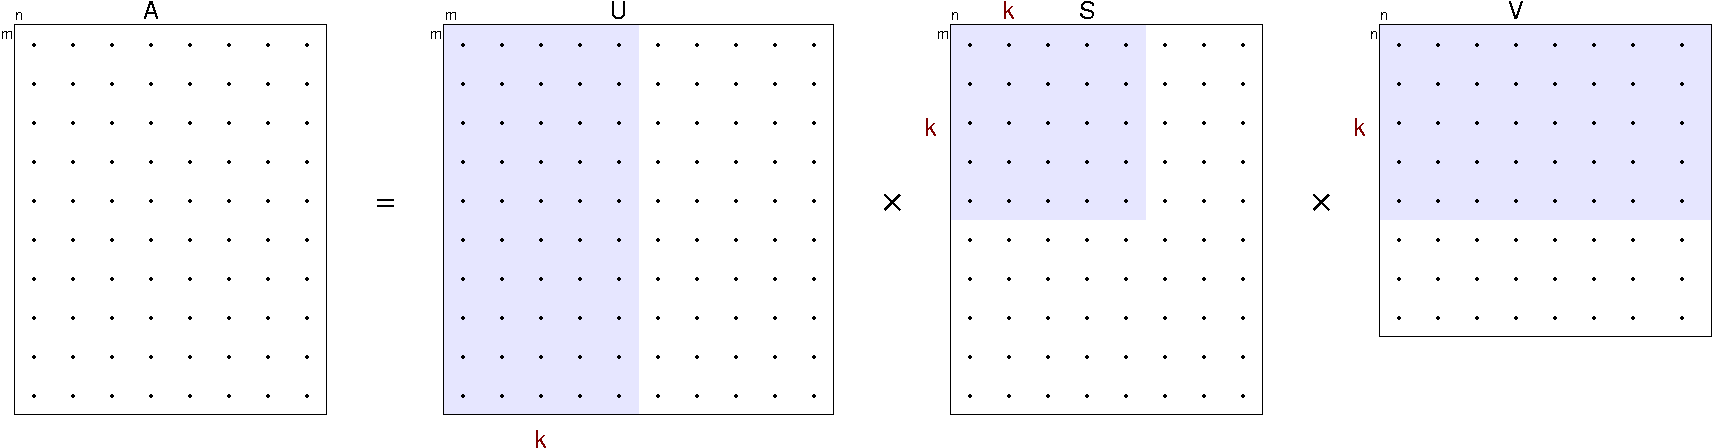
\includegraphics[width=\linewidth]{svdmatrixk}
    \end{overprint}
\end{frame}

\begin{frame}
    \frametitle{An example}
    \centering
    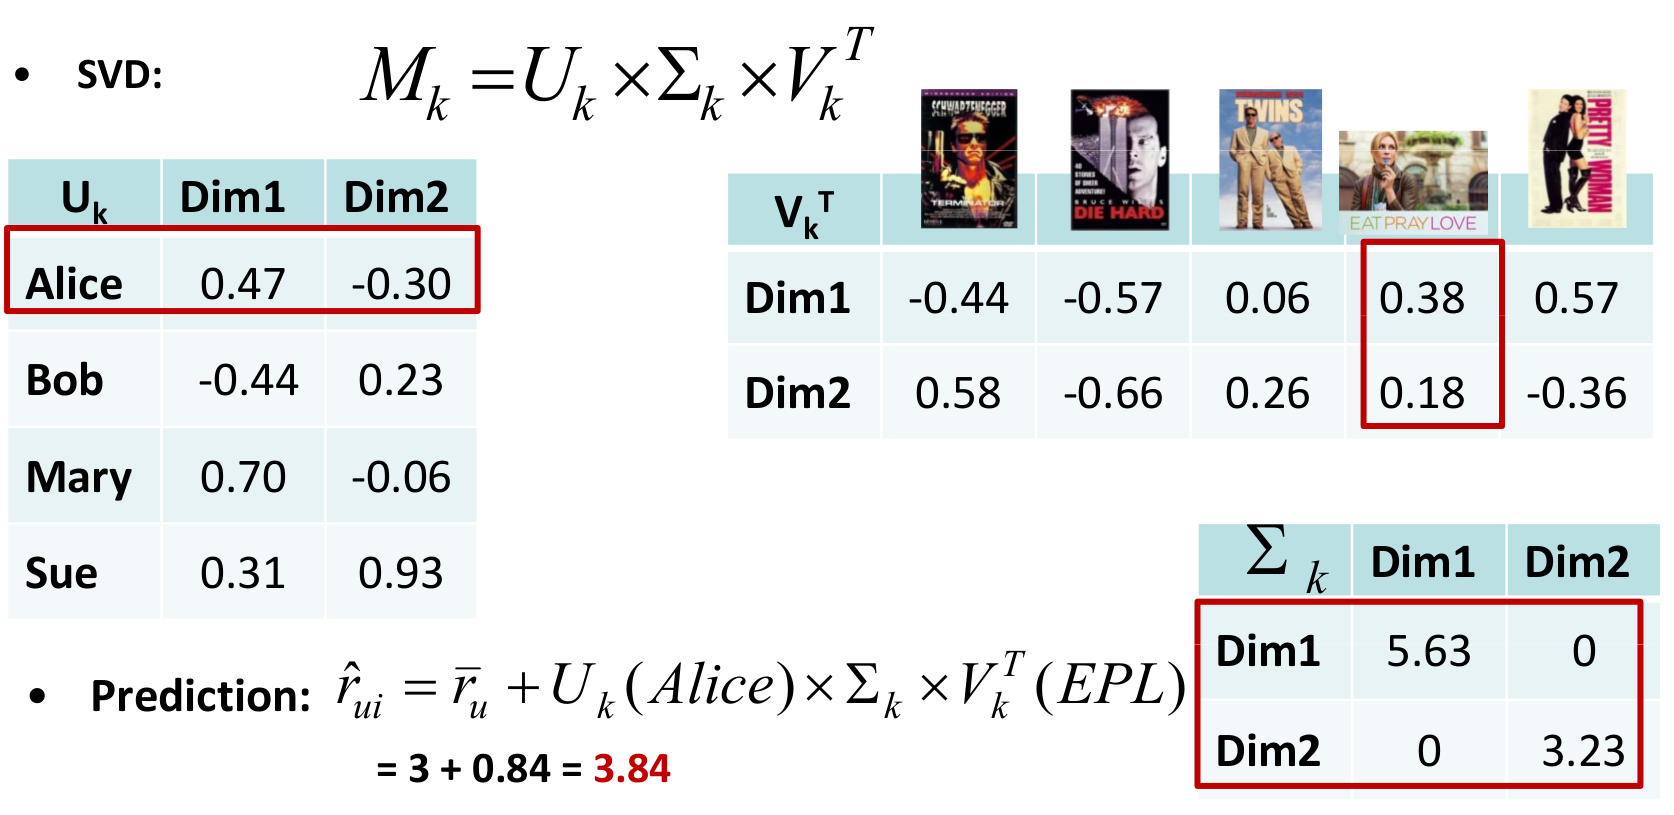
\includegraphics[width=\linewidth]{svdalice}
\end{frame}

\begin{frame}
    \frametitle{The low dimensional space}
    \centering
    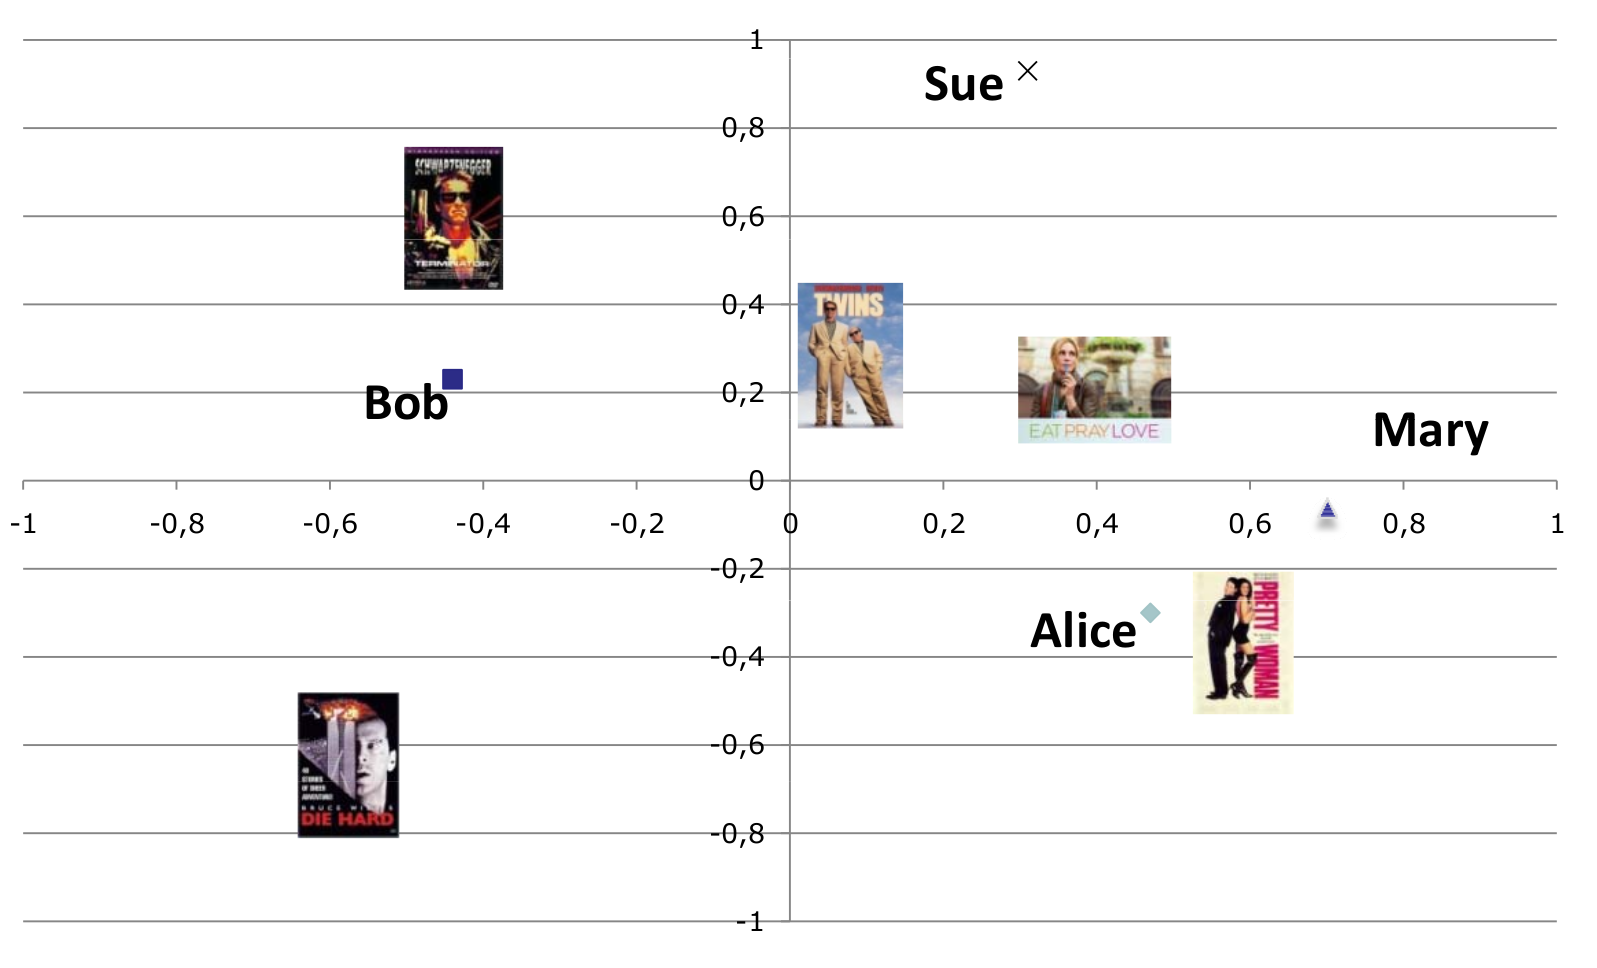
\includegraphics[width=\linewidth]{svdpic}
\end{frame}

\section{Content-based Filtering}

\begin{frame}
    \frametitle{Content-based recommendation}
    \begin{itemize}
    \item While CF methods do not require any information about the items
        \begin{itemize}
        \item it might be reasonable to exploit such information; and
        \item e.g. recommend fantasy novels to people who liked fantasy novels
            in the past
        \end{itemize}
    \item What do we need:
        \begin{itemize}
        \item some information about the available items such as the genre
            (\emph{content})
        \item some sort of user profile describing what the user likes
            (\emph{preferences})
        \end{itemize}
    \item The task:
        \begin{itemize}
        \item learn user preferences
        \item recommend items that are \emph{similar to the user preferences}
        \end{itemize}
    \end{itemize}
\end{frame}

\begin{frame}
    \frametitle{Content Representation and Item Similarities}
    \hfill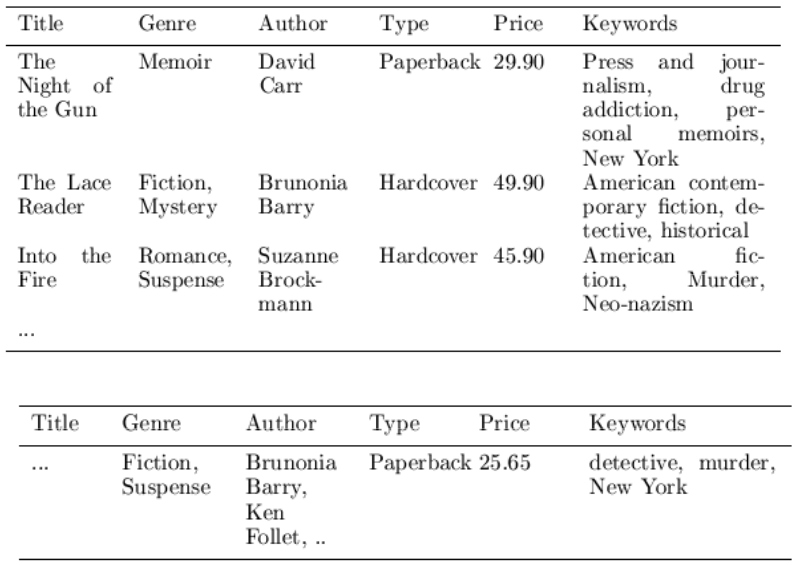
\includegraphics[width=.8\linewidth]{content}\hfill~ \\
    \begin{itemize}
    \item {Simple approach:} compute the similarity between the user profile
        and an unseen item using keyword overlap
        \begin{itemize}
        \item E.g. use the \emph{vector space model} (from IR)
        \end{itemize}
    \end{itemize}
\end{frame}

\begin{frame}
    \frametitle{Recommending Items}
    \begin{itemize}
    \item Simple method: \emph{nearest neighbors}
        \begin{itemize}
        \item Given a set of documents $D$ already rated by the user
            (like/dislike)
            \begin{itemize}
            \item Find the $n$ nearest neighbors of a not-yet-seen item $i \in
                D$
            \item Take these ratings to predict a rating/vote for $i$
            \end{itemize}
        \item Good to model short-term interests/follow-up stories
        \item Used in combination with method to model long-term preferences
        \end{itemize}
    \item Query-based retrieval: \emph{Rocchio's method}
        \begin{itemize}
        \item Users are allowed to rate (relevant/irrelevant) retrieved
            documents (feedback)
        \item The system then learns a prototype of relevant/irrelevant
            documents
        \item Queries are then automatically extended with additional
            terms/weight of relevant documents
        \end{itemize}
    \end{itemize}
\end{frame}

\begin{frame}
    \frametitle{Rocchio Relevance Feedback Method}
    \begin{block}{}
        \begin{displaymath}
            Q_{i+1} = \alpha \times Q_i + \beta (\frac{1}{|D^+|}\sum_{d^+\in
              D^+}d^+) - \gamma (\frac{1}{|D^-|}\sum_{d^-\in D^-}d^-)
        \end{displaymath}
        \centering
        \begin{minipage}{0.7\linewidth}
            $D^+, D^-$: positive/negative items\\
            $Q$: query\\
            $\alpha, \beta, \gamma$: used to fine tune the process
        \end{minipage}
    \end{block}
\end{frame}

\begin{frame}
    \frametitle{Other Methods}
    \begin{itemize}
    \item Classifiers
        \begin{itemize}
        \item E.g. using 2 classes: relevant/non-relevant
        \end{itemize}
    \item Other information retrieval methods
        \begin{itemize}
        \item As used by search engines (L2R, PageRank, etc.)
        \end{itemize}
    \end{itemize}
\end{frame}

\begin{frame}
    \frametitle{Limitations of Content-based Recommendation Methods}
    \begin{itemize}
    \item Keywords alone may not be sufficient to judge quality/relevance of a
        document or web page
        \begin{itemize}
        \item content may be limited/too short
        \item content may not be automatically extractable (e.g. multimedia)
        \end{itemize}
    \item Ramp-up phase required
        \begin{itemize}
        \item Some training data is still required
        \end{itemize}
    \item Over-specialization
        \begin{itemize}
        \item Algorithms tend to propose ``more of the same''
        \item E.g. different news items about the same news story
        \end{itemize}
    \end{itemize}
\end{frame}

\section{Knowledge-based Recommendation}

\begin{frame}
    \frametitle{Knowledge-Based Recommendation}
    \begin{itemize}
    \item Explicit domain knowledge
        \begin{itemize}
        \item Requirements elicitation from domain experts
        \item System mimics the behavior of experienced sales assistant
        \item Can guarantee ``correct'' recommendations (determinism) with
            respect to expert knowledge
        \end{itemize}
    \item Conversational interaction strategy
        \begin{itemize}
        \item Opposed to one-shot interaction
        \item Elicitation of user requirements
        \item Transfer of product knowledge (``educating users'')
        \end{itemize}
    \end{itemize}
\end{frame}

\begin{frame}
    \frametitle{Constraint-based Recommendation}
    \begin{itemize}
    \item \emph{Knowledge base}
        \begin{itemize}
        \item Usually mediates between user model and item properties
        \item Variables
            \begin{itemize}
            \item User model features (\emph{requirements}), item features
                (\emph{catalogue})
            \end{itemize}
        \end{itemize}
    \item Set of constraints
        \begin{itemize}
        \item Logical implications (\texttt{IF} user requires $A$ \texttt{THEN}
            proposed item should possess feature $B$)
        \item Hard and soft/weighted constraints
        \item Solution preferences
        \end{itemize}
    \item Derive a set of recommendable items
        \begin{itemize}
        \item Fulfilling a set of applicable constraints
        \item Applicability of constraints depends on current user model
        \item \emph{Explanations:} transparent line of reasoning
        \end{itemize}
    \end{itemize}
\end{frame}

\begin{frame}
    \frametitle{Example}
    \footnotesize
    \begin{columns}
        \column{.5\linewidth}
        \begin{block}{Knowledge base}
            \ttfamily
            True $\Rightarrow$ brand = brand prefs\\
            Motives = Landscape $\Rightarrow$ \\
            \hfill Low foc Length $\leq$ 28\\
            True $\Rightarrow$ Price $\leq$ Max cost\\
            ...
        \end{block}
        \begin{block}{User model}
            \ttfamily
            Motives = Landscape\\
            Brand pref = Canon\\
            Max cost = 350
        \end{block}
        \column{.4\linewidth}
        \begin{block}{Catalogue}
            \centering
            \fbox{
              \begin{minipage}{.8\linewidth}
                  \ttfamily
                  Brand = Canon\\
                  Low foc length = 35\\
                  Up foc length = 140\\
                  Price = 420
              \end{minipage}}\\\vsep
            \fbox{
              \begin{minipage}{.8\linewidth}
                  \ttfamily
                  Brand = Panasonic\\
                  Low foc length = 28\\
                  Up foc length = 112\\
                  Price = 319
              \end{minipage}}\\[\baselineskip]
            ...
        \end{block}
    \end{columns}
\end{frame}

\begin{frame}
    \frametitle{Conversational Strategies}
    \footnotesize
    \begin{columns}
        \column{.5\linewidth}
        \begin{itemize}
        \item Process consisting of multiple conversational moves
            \begin{itemize}
                \footnotesize
            \item Resembles natural sales interactions
            \item Not all user requirements known beforehand
            \item Customers are rarely satisfied with the initial
                recommendations
            \end{itemize}
        \item Different styles of preference elicitation:
            \begin{itemize}
                \footnotesize
            \item Free text query interface
            \item Asking technical/generic properties
            \item Images/inspiration
            \item Proposing and Critiquing
            \end{itemize}
        \end{itemize}
        \column{.5\linewidth}
        \centering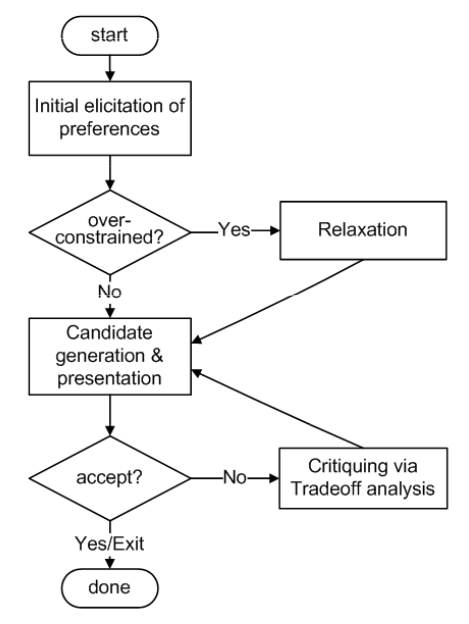
\includegraphics[width=\linewidth]{dialogue}
    \end{columns}
\end{frame}

\begin{frame}
    \frametitle{Limitations of Knowledge-based Recommendation Methods}
    \begin{itemize}
    \item Cost of knowledge acquisition
        \begin{itemize}
        \item From domain experts
        \item From users
        \item From web resources
        \end{itemize}
    \item Accuracy of preference models
        \begin{itemize}
        \item Very fine granular preference models require many interaction
            cycles with the user or sufficient detailed data about the user
        \item Whereas collaborative filtering models the preference of a user
            implicitly
        \end{itemize}
    \item Independence and stability assumption can be challenged
        \begin{itemize}
        \item Preferences are not always independent from each other and stable
        \end{itemize}
    \end{itemize}
\end{frame}

\section{Hybrid Strategies}

\begin{frame}
    \frametitle{Hybrid Recommender Systems}
    Different hybridization designs 
    \begin{itemize}
    \item Monolithic exploiting different features
    \item Parallel use of several systems
    \item Pipelined invocation of different systems
    \end{itemize}
\end{frame}

\begin{frame}
    \frametitle{Monolithic Hybridization Design}
    \begin{itemize}
    \item Only a single recommendation component\\
        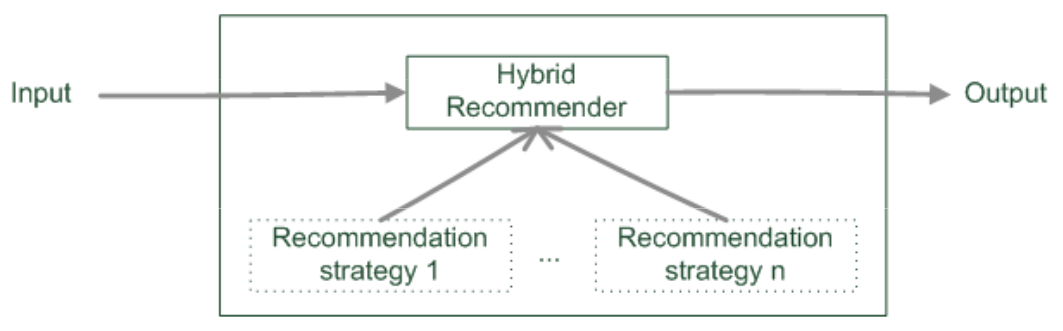
\includegraphics[width=\linewidth]{mono}
    \item Combination of several knowledge sources
        \begin{itemize}
        \item E.g. ratings and user demographics or explicit requirements and
            needs used for similarity computation
        \end{itemize}
    \item \emph{Hybrid} features:
        \begin{itemize}
        \item Social features: Movies liked by user
        \item Content features: Comedies liked by user, dramas liked by user
        \end{itemize}
    \end{itemize}
\end{frame}

\begin{frame}
    \frametitle{Parallelized Hybridization Design}
    \begin{itemize}
    \item Output of several existing implementations combined
    \item Least invasive design
    \item Weighting or voting scheme applied\\
        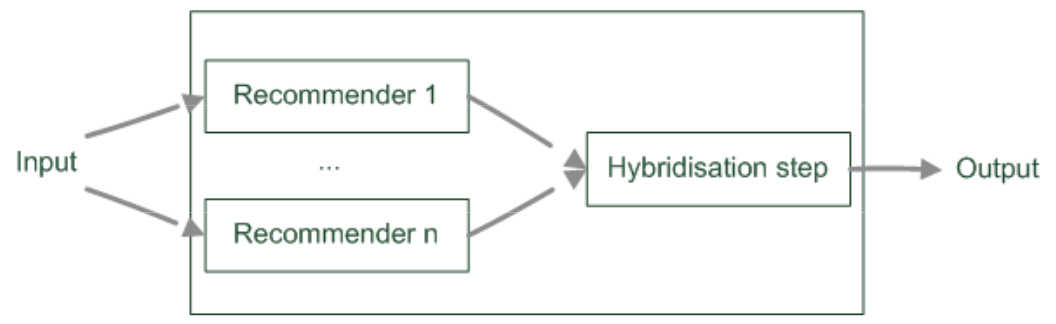
\includegraphics[width=\linewidth]{paralel}
        \begin{itemize}
        \item Weights can be learned dynamically
        \end{itemize}
    \end{itemize}
\end{frame}

\begin{frame}
    \frametitle{Pipelined hybridization designs}
    One recommender system pre-processes some input for the subsequent
    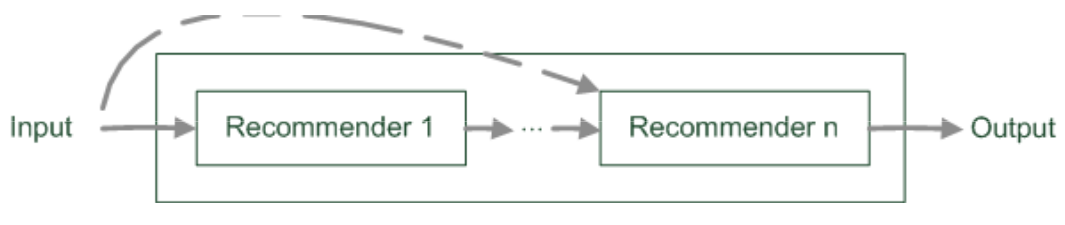
\includegraphics[width=\linewidth]{pipeline}
    \begin{itemize}
    \item \emph{Cascade:} Refinement of recommendation lists
        \begin{itemize}
        \item E.g. first recommender excludes items (e.g. knowledge-based);
            second recommender assigns score (e.g. collaborative)
        \end{itemize}
    \item \emph{Meta-level:} Learning of model
        \begin{itemize}
        \item E.g. collaborative filtering identifies similar users; knowledge
            base is built using behavior of similar users
        \end{itemize}
    \end{itemize}
\end{frame}

\begin{frame}
    \frametitle{Limitations and Success of Hybridization Strategies}
    \begin{itemize}
    \item Most datasets do not allow to compare different recommendation
        paradigms
        \begin{itemize}
        \item i.e. ratings, requirements, item features, domain knowledge,
            critiques rarely available in a single dataset
        \end{itemize}
    \item Thus few conclusions that are supported by empirical findings
        % \begin{itemize}
        % \item Monolithic: some preprocessing effort traded-in for more
        %     knowledge included
        % \item Parallel: requires careful matching of scores from different
        %     predictors
        % \item Pipelined: works well for two antithetic approaches
        % \end{itemize}
    \item Netflix competition---stacking recommender systems
        \begin{itemize}
        \item Weighted design based on $>100$ predictors (recommendation
            functions)
        % \item Adaptive switching of weights based on user model, parameters
        %     (e.g. number of ratings in one session)
        \end{itemize}
    \end{itemize}
\end{frame}

\section{Summary}

\begin{frame}
    \frametitle{Pros \& Cons}    
    \centering
    \vsep
    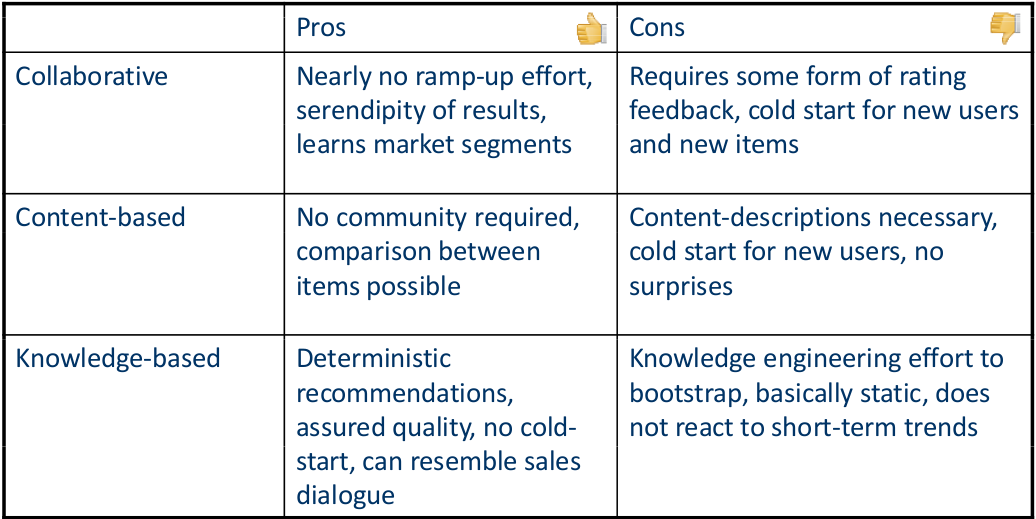
\includegraphics[width=\linewidth]{techniques}
\end{frame}

\begin{frame}
    \frametitle{Other Topics}
    \begin{itemize}
    \item Explanations
        \begin{itemize}
        \item A selling agent may be interested in promoting particular
            products
        \item A buying agent is concerned about making the right buying
            decision
        \end{itemize}
    \item Evaluation
        \begin{itemize}
        \item Common metrics: \emph{precision}, \emph{recall}, \emph{F1}, etc.
        \item However: real-value lies in increasing conversions and
            satisfaction with bought items (low churn rate)
        \end{itemize}
    \end{itemize}
\end{frame}

% ------------------------------------------------------------

\finalframe{Questions?}

\end{document}
